\documentclass[]{article}
\usepackage{lmodern}
\usepackage{amssymb,amsmath}
\usepackage{ifxetex,ifluatex}
\usepackage{fixltx2e} % provides \textsubscript
\ifnum 0\ifxetex 1\fi\ifluatex 1\fi=0 % if pdftex
  \usepackage[T1]{fontenc}
  \usepackage[utf8]{inputenc}
\else % if luatex or xelatex
  \ifxetex
    \usepackage{mathspec}
  \else
    \usepackage{fontspec}
  \fi
  \defaultfontfeatures{Ligatures=TeX,Scale=MatchLowercase}
\fi
% use upquote if available, for straight quotes in verbatim environments
\IfFileExists{upquote.sty}{\usepackage{upquote}}{}
% use microtype if available
\IfFileExists{microtype.sty}{%
\usepackage{microtype}
\UseMicrotypeSet[protrusion]{basicmath} % disable protrusion for tt fonts
}{}
\usepackage[margin=1in]{geometry}
\usepackage{hyperref}
\hypersetup{unicode=true,
            pdftitle={Reproducible Report Template - Basic},
            pdfauthor={Student(s) SID},
            pdfborder={0 0 0},
            breaklinks=true}
\urlstyle{same}  % don't use monospace font for urls
\usepackage{color}
\usepackage{fancyvrb}
\newcommand{\VerbBar}{|}
\newcommand{\VERB}{\Verb[commandchars=\\\{\}]}
\DefineVerbatimEnvironment{Highlighting}{Verbatim}{commandchars=\\\{\}}
% Add ',fontsize=\small' for more characters per line
\usepackage{framed}
\definecolor{shadecolor}{RGB}{248,248,248}
\newenvironment{Shaded}{\begin{snugshade}}{\end{snugshade}}
\newcommand{\AlertTok}[1]{\textcolor[rgb]{0.94,0.16,0.16}{#1}}
\newcommand{\AnnotationTok}[1]{\textcolor[rgb]{0.56,0.35,0.01}{\textbf{\textit{#1}}}}
\newcommand{\AttributeTok}[1]{\textcolor[rgb]{0.77,0.63,0.00}{#1}}
\newcommand{\BaseNTok}[1]{\textcolor[rgb]{0.00,0.00,0.81}{#1}}
\newcommand{\BuiltInTok}[1]{#1}
\newcommand{\CharTok}[1]{\textcolor[rgb]{0.31,0.60,0.02}{#1}}
\newcommand{\CommentTok}[1]{\textcolor[rgb]{0.56,0.35,0.01}{\textit{#1}}}
\newcommand{\CommentVarTok}[1]{\textcolor[rgb]{0.56,0.35,0.01}{\textbf{\textit{#1}}}}
\newcommand{\ConstantTok}[1]{\textcolor[rgb]{0.00,0.00,0.00}{#1}}
\newcommand{\ControlFlowTok}[1]{\textcolor[rgb]{0.13,0.29,0.53}{\textbf{#1}}}
\newcommand{\DataTypeTok}[1]{\textcolor[rgb]{0.13,0.29,0.53}{#1}}
\newcommand{\DecValTok}[1]{\textcolor[rgb]{0.00,0.00,0.81}{#1}}
\newcommand{\DocumentationTok}[1]{\textcolor[rgb]{0.56,0.35,0.01}{\textbf{\textit{#1}}}}
\newcommand{\ErrorTok}[1]{\textcolor[rgb]{0.64,0.00,0.00}{\textbf{#1}}}
\newcommand{\ExtensionTok}[1]{#1}
\newcommand{\FloatTok}[1]{\textcolor[rgb]{0.00,0.00,0.81}{#1}}
\newcommand{\FunctionTok}[1]{\textcolor[rgb]{0.00,0.00,0.00}{#1}}
\newcommand{\ImportTok}[1]{#1}
\newcommand{\InformationTok}[1]{\textcolor[rgb]{0.56,0.35,0.01}{\textbf{\textit{#1}}}}
\newcommand{\KeywordTok}[1]{\textcolor[rgb]{0.13,0.29,0.53}{\textbf{#1}}}
\newcommand{\NormalTok}[1]{#1}
\newcommand{\OperatorTok}[1]{\textcolor[rgb]{0.81,0.36,0.00}{\textbf{#1}}}
\newcommand{\OtherTok}[1]{\textcolor[rgb]{0.56,0.35,0.01}{#1}}
\newcommand{\PreprocessorTok}[1]{\textcolor[rgb]{0.56,0.35,0.01}{\textit{#1}}}
\newcommand{\RegionMarkerTok}[1]{#1}
\newcommand{\SpecialCharTok}[1]{\textcolor[rgb]{0.00,0.00,0.00}{#1}}
\newcommand{\SpecialStringTok}[1]{\textcolor[rgb]{0.31,0.60,0.02}{#1}}
\newcommand{\StringTok}[1]{\textcolor[rgb]{0.31,0.60,0.02}{#1}}
\newcommand{\VariableTok}[1]{\textcolor[rgb]{0.00,0.00,0.00}{#1}}
\newcommand{\VerbatimStringTok}[1]{\textcolor[rgb]{0.31,0.60,0.02}{#1}}
\newcommand{\WarningTok}[1]{\textcolor[rgb]{0.56,0.35,0.01}{\textbf{\textit{#1}}}}
\usepackage{graphicx,grffile}
\makeatletter
\def\maxwidth{\ifdim\Gin@nat@width>\linewidth\linewidth\else\Gin@nat@width\fi}
\def\maxheight{\ifdim\Gin@nat@height>\textheight\textheight\else\Gin@nat@height\fi}
\makeatother
% Scale images if necessary, so that they will not overflow the page
% margins by default, and it is still possible to overwrite the defaults
% using explicit options in \includegraphics[width, height, ...]{}
\setkeys{Gin}{width=\maxwidth,height=\maxheight,keepaspectratio}
\IfFileExists{parskip.sty}{%
\usepackage{parskip}
}{% else
\setlength{\parindent}{0pt}
\setlength{\parskip}{6pt plus 2pt minus 1pt}
}
\setlength{\emergencystretch}{3em}  % prevent overfull lines
\providecommand{\tightlist}{%
  \setlength{\itemsep}{0pt}\setlength{\parskip}{0pt}}
\setcounter{secnumdepth}{0}
% Redefines (sub)paragraphs to behave more like sections
\ifx\paragraph\undefined\else
\let\oldparagraph\paragraph
\renewcommand{\paragraph}[1]{\oldparagraph{#1}\mbox{}}
\fi
\ifx\subparagraph\undefined\else
\let\oldsubparagraph\subparagraph
\renewcommand{\subparagraph}[1]{\oldsubparagraph{#1}\mbox{}}
\fi

%%% Use protect on footnotes to avoid problems with footnotes in titles
\let\rmarkdownfootnote\footnote%
\def\footnote{\protect\rmarkdownfootnote}

%%% Change title format to be more compact
\usepackage{titling}

% Create subtitle command for use in maketitle
\providecommand{\subtitle}[1]{
  \posttitle{
    \begin{center}\large#1\end{center}
    }
}

\setlength{\droptitle}{-2em}

  \title{Reproducible Report Template - Basic}
    \pretitle{\vspace{\droptitle}\centering\huge}
  \posttitle{\par}
  \subtitle{Project X}
  \author{Student(s) SID}
    \preauthor{\centering\large\emph}
  \postauthor{\par}
      \predate{\centering\large\emph}
  \postdate{\par}
    \date{University of Sydney \textbar{} Unit of Study \textbar{} Month Year}


\begin{document}
\maketitle

{
\setcounter{tocdepth}{3}
\tableofcontents
}
\begin{Shaded}
\begin{Highlighting}[]
\KeywordTok{library}\NormalTok{(ggplot2)}
\KeywordTok{library}\NormalTok{(dplyr)}
\end{Highlighting}
\end{Shaded}

\begin{verbatim}
## 
## Attaching package: 'dplyr'
\end{verbatim}

\begin{verbatim}
## The following objects are masked from 'package:stats':
## 
##     filter, lag
\end{verbatim}

\begin{verbatim}
## The following objects are masked from 'package:base':
## 
##     intersect, setdiff, setequal, union
\end{verbatim}

\begin{Shaded}
\begin{Highlighting}[]
\KeywordTok{library}\NormalTok{(readr)}
\NormalTok{master <-}\StringTok{ }\KeywordTok{read_csv}\NormalTok{(}\StringTok{"/Users/zhanghaochen/Downloads/data/master.csv"}\NormalTok{)}
\end{Highlighting}
\end{Shaded}

\begin{verbatim}
## Parsed with column specification:
## cols(
##   Signum = col_character(),
##   Plats = col_character(),
##   Socken = col_character(),
##   Härad = col_character(),
##   Kommun = col_character(),
##   KoordinaterX = col_double(),
##   KoordinaterY = col_double(),
##   Stilgruppering = col_character(),
##   Ristare = col_character(),
##   Materialtyp = col_character(),
##   Bildlänk = col_character()
## )
\end{verbatim}

\begin{verbatim}
## Warning: 906 parsing failures.
##  row          col               expected actual                                            file
## 3233 KoordinaterX a double                 (55  '/Users/zhanghaochen/Downloads/data/master.csv'
## 3233 KoordinaterY no trailing characters    ; 9 '/Users/zhanghaochen/Downloads/data/master.csv'
## 3235 KoordinaterX a double                 (55  '/Users/zhanghaochen/Downloads/data/master.csv'
## 3235 KoordinaterY no trailing characters    ; 9 '/Users/zhanghaochen/Downloads/data/master.csv'
## 3242 KoordinaterX a double                 (55  '/Users/zhanghaochen/Downloads/data/master.csv'
## .... ............ ...................... ...... ...............................................
## See problems(...) for more details.
\end{verbatim}

\begin{Shaded}
\begin{Highlighting}[]
\KeywordTok{library}\NormalTok{(readr)}
\NormalTok{master_church <-}\StringTok{ }\KeywordTok{read_csv}\NormalTok{(}\StringTok{"/Users/zhanghaochen/Downloads/data/未命名文件夹/master_church.csv"}\NormalTok{)}
\end{Highlighting}
\end{Shaded}

\begin{verbatim}
## Parsed with column specification:
## cols(
##   Signum = col_character(),
##   Plats = col_character(),
##   Socken = col_character(),
##   Härad = col_character(),
##   Kommun = col_character(),
##   KoordinaterX = col_double(),
##   KoordinaterY = col_double(),
##   Stilgruppering = col_character(),
##   Ristare = col_character(),
##   Materialtyp = col_character()
## )
\end{verbatim}

\begin{verbatim}
## Warning: 1 parsing failure.
##  row          col               expected actual                                                                file
## 1276 KoordinaterY no trailing characters   ; 15 '/Users/zhanghaochen/Downloads/data/未命名文件夹/master_church.csv'
\end{verbatim}

\begin{Shaded}
\begin{Highlighting}[]
\KeywordTok{library}\NormalTok{(readr)}
\NormalTok{master_churchyard <-}\StringTok{ }\KeywordTok{read_csv}\NormalTok{(}\StringTok{"/Users/zhanghaochen/Downloads/data/未命名文件夹/master_churchyard.csv"}\NormalTok{)}
\end{Highlighting}
\end{Shaded}

\begin{verbatim}
## Parsed with column specification:
## cols(
##   Signum = col_character(),
##   Plats = col_character(),
##   Socken = col_character(),
##   Härad = col_character(),
##   Kommun = col_character(),
##   KoordinaterX = col_double(),
##   KoordinaterY = col_double(),
##   Stilgruppering = col_character(),
##   Ristare = col_character(),
##   Materialtyp = col_character()
## )
\end{verbatim}

\hypertarget{executive-summary}{%
\section{Executive Summary}\label{executive-summary}}

\hypertarget{full-report}{%
\section{Full Report}\label{full-report}}

\hypertarget{initial-data-analysis-ida}{%
\subsection{Initial Data Analysis
(IDA)}\label{initial-data-analysis-ida}}

\begin{Shaded}
\begin{Highlighting}[]
\NormalTok{p_select=master }\OperatorTok
\KeywordTok{select}\NormalTok{(Signum,KoordinaterX,KoordinaterY,Stilgruppering)}
\NormalTok{p_select_}\DecValTok{1}\NormalTok{=p_select }\OperatorTok
\KeywordTok{filter}\NormalTok{(Stilgruppering}\OperatorTok{==}\StringTok{'RAK'} \OperatorTok{|}\StringTok{ }\NormalTok{Stilgruppering}\OperatorTok{==}\StringTok{'Pr2'} \OperatorTok{|}\NormalTok{Stilgruppering}\OperatorTok{==}\StringTok{'Pr3'} \OperatorTok{|}\NormalTok{Stilgruppering}\OperatorTok{==}\StringTok{'Pr4'}\OperatorTok{|}\NormalTok{Stilgruppering}\OperatorTok{==}\StringTok{'Pr5'}\OperatorTok{|}\NormalTok{Stilgruppering}\OperatorTok{==}\StringTok{'FP'}\OperatorTok{|}\NormalTok{Stilgruppering}\OperatorTok{==}\StringTok{'Pr1'}\OperatorTok{|}\NormalTok{Stilgruppering}\OperatorTok{==}\StringTok{'Pr1 - Pr2?'}\OperatorTok{|}\NormalTok{Stilgruppering}\OperatorTok{==}\StringTok{'Pr2 - Pr3?'}\OperatorTok{|}\NormalTok{Stilgruppering}\OperatorTok{==}\StringTok{'Pr3 - Pr4?'}\OperatorTok{|}\NormalTok{Stilgruppering}\OperatorTok{==}\StringTok{'Pr4 - Pr5?'}\NormalTok{)}
\NormalTok{p_plot=}\KeywordTok{ggplot}\NormalTok{(p_select_}\DecValTok{1}\NormalTok{,}\KeywordTok{aes}\NormalTok{(KoordinaterX,KoordinaterY))}
\NormalTok{p_plot}\OperatorTok{+}\KeywordTok{geom_point}\NormalTok{(}\KeywordTok{aes}\NormalTok{(}\DataTypeTok{color=}\NormalTok{Stilgruppering))}
\end{Highlighting}
\end{Shaded}

\begin{verbatim}
## Warning: Removed 162 rows containing missing values (geom_point).
\end{verbatim}

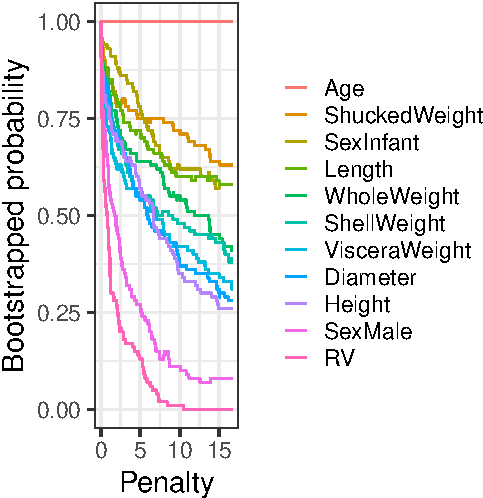
\includegraphics{ReportTemplateBasic1_files/figure-latex/unnamed-chunk-2-1.pdf}

\begin{Shaded}
\begin{Highlighting}[]
\NormalTok{rune_stone2=}\KeywordTok{data.frame}\NormalTok{(}\StringTok{"sum"}\NormalTok{=}\KeywordTok{c}\NormalTok{(}\DecValTok{452}\NormalTok{,}\DecValTok{76}\NormalTok{,}\DecValTok{83}\NormalTok{,}\DecValTok{227}\NormalTok{,}\DecValTok{51}\NormalTok{,}\DecValTok{6}\NormalTok{,}\DecValTok{11}\NormalTok{,}\DecValTok{27}\NormalTok{,}\DecValTok{33}\NormalTok{,}\DecValTok{627}\NormalTok{,}\DecValTok{195}\NormalTok{,}\DecValTok{147}\NormalTok{,}\DecValTok{10}\NormalTok{,}\DecValTok{109}\NormalTok{,}\DecValTok{16}\NormalTok{,}\DecValTok{11}\NormalTok{,}\DecValTok{36}\NormalTok{,}\DecValTok{13}\NormalTok{,}\DecValTok{186}\NormalTok{,}\DecValTok{196}\NormalTok{,}\DecValTok{159}\NormalTok{,}\DecValTok{238}\NormalTok{,}\DecValTok{146}\NormalTok{,}\DecValTok{797}\NormalTok{,}\DecValTok{36}\NormalTok{,}\DecValTok{57}\NormalTok{,}\DecValTok{63}\NormalTok{,}\DecValTok{30}\NormalTok{,}\DecValTok{7}\NormalTok{,}\DecValTok{33}\NormalTok{,}\DecValTok{28}\NormalTok{,}\DecValTok{190}\NormalTok{,}\DecValTok{43}\NormalTok{,}\DecValTok{54}\NormalTok{,}\DecValTok{65}\NormalTok{,}\DecValTok{85}\NormalTok{,}\DecValTok{19}\NormalTok{,}\DecValTok{57}\NormalTok{,}\DecValTok{9}\NormalTok{,}\DecValTok{37}\NormalTok{,}\DecValTok{62}\NormalTok{,}\DecValTok{52}\NormalTok{,}\DecValTok{913}\NormalTok{,}\DecValTok{3}\NormalTok{,}\DecValTok{1}\NormalTok{,}\DecValTok{12}\NormalTok{),}\StringTok{"name"}\NormalTok{=}\KeywordTok{c}\NormalTok{(}\StringTok{"A1"}\NormalTok{,}\StringTok{"A2"}\NormalTok{,}\StringTok{"A3"}\NormalTok{,}\StringTok{"A4"}\NormalTok{,}\StringTok{"A5"}\NormalTok{,}\StringTok{"A6"}\NormalTok{,}\StringTok{"A7"}\NormalTok{,}\StringTok{"A8"}\NormalTok{,}\StringTok{"A9"}\NormalTok{,}\StringTok{"B1"}\NormalTok{,}\StringTok{"B2"}\NormalTok{,}\StringTok{"B3"}\NormalTok{,}\StringTok{"B4"}\NormalTok{,}\StringTok{"C1"}\NormalTok{,}\StringTok{"C2"}\NormalTok{,}\StringTok{"C3"}\NormalTok{,}\StringTok{"C4"}\NormalTok{,}\StringTok{"C5"}\NormalTok{,}\StringTok{"C6"}\NormalTok{,}\StringTok{"C7"}\NormalTok{,}\StringTok{"C8"}\NormalTok{,}\StringTok{"C9"}\NormalTok{,}\StringTok{"C10"}\NormalTok{,}\StringTok{"D1"}\NormalTok{,}\StringTok{"D2"}\NormalTok{,}\StringTok{"D3"}\NormalTok{,}\StringTok{"D4"}\NormalTok{,}\StringTok{"D5"}\NormalTok{,}\StringTok{"D6"}\NormalTok{,}\StringTok{"E1"}\NormalTok{,}\StringTok{"E2"}\NormalTok{,}\StringTok{"E3"}\NormalTok{,}\StringTok{"E4"}\NormalTok{,}\StringTok{"E5"}\NormalTok{,}\StringTok{"E6"}\NormalTok{,}\StringTok{"E7"}\NormalTok{,}\StringTok{"E8"}\NormalTok{,}\StringTok{"E9"}\NormalTok{,}\StringTok{"E10"}\NormalTok{,}\StringTok{"E11"}\NormalTok{,}\StringTok{"F1"}\NormalTok{,}\StringTok{"F2"}\NormalTok{,}\StringTok{"F3"}\NormalTok{,}\StringTok{"F4"}\NormalTok{,}\StringTok{"G1"}\NormalTok{,}\StringTok{"G2"}\NormalTok{),}\DataTypeTok{stringsAsFactors =} \OtherTok{FALSE}\NormalTok{)}
\NormalTok{p_sum=}\KeywordTok{ggplot}\NormalTok{(rune_stone2,}\KeywordTok{aes}\NormalTok{(name,sum))}
\NormalTok{p_sum}\OperatorTok{+}\KeywordTok{geom_point}\NormalTok{(}\KeywordTok{aes}\NormalTok{(}\DataTypeTok{color=}\NormalTok{name))}
\end{Highlighting}
\end{Shaded}

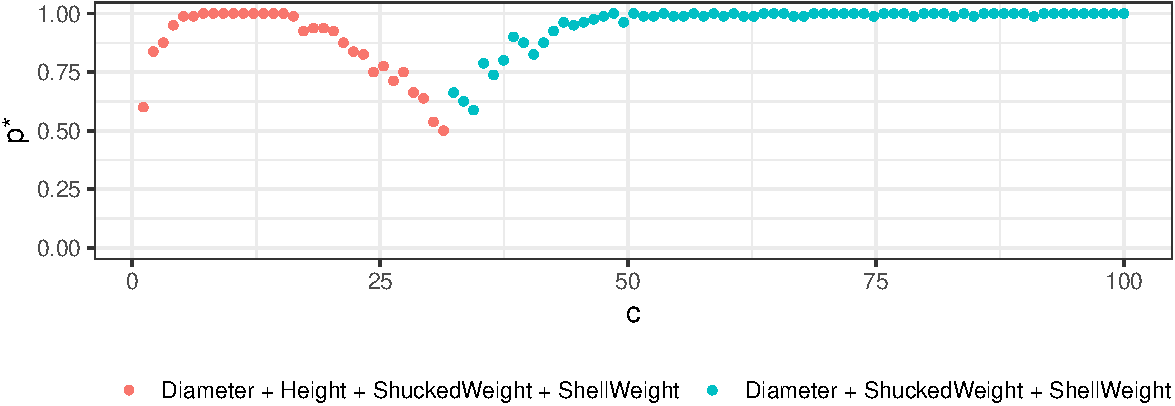
\includegraphics{ReportTemplateBasic1_files/figure-latex/unnamed-chunk-3-1.pdf}

\begin{Shaded}
\begin{Highlighting}[]
\NormalTok{p_select_church=}\StringTok{ }\NormalTok{master_church }\OperatorTok
\KeywordTok{select}\NormalTok{(Plats,KoordinaterX,KoordinaterY,Stilgruppering)}
\NormalTok{p_select_church1=p_select_church }\OperatorTok
\KeywordTok{filter}\NormalTok{(Stilgruppering}\OperatorTok{==}\StringTok{'RAK'} \OperatorTok{|}\StringTok{ }\NormalTok{Stilgruppering}\OperatorTok{==}\StringTok{'Pr2'} \OperatorTok{|}\NormalTok{Stilgruppering}\OperatorTok{==}\StringTok{'Pr3'} \OperatorTok{|}\NormalTok{Stilgruppering}\OperatorTok{==}\StringTok{'Pr4'}\OperatorTok{|}\NormalTok{Stilgruppering}\OperatorTok{==}\StringTok{'Pr5'}\OperatorTok{|}\NormalTok{Stilgruppering}\OperatorTok{==}\StringTok{'FP'}\OperatorTok{|}\NormalTok{Stilgruppering}\OperatorTok{==}\StringTok{'Pr1'}\NormalTok{) }
\NormalTok{count_church=}\KeywordTok{table}\NormalTok{(p_select_church1}\OperatorTok{$}\NormalTok{Stilgruppering)}
\KeywordTok{barplot}\NormalTok{(count_church, }\DataTypeTok{main=}\StringTok{"stone in church"}\NormalTok{,}\DataTypeTok{xlab=}\StringTok{"period"}\NormalTok{)}
\end{Highlighting}
\end{Shaded}

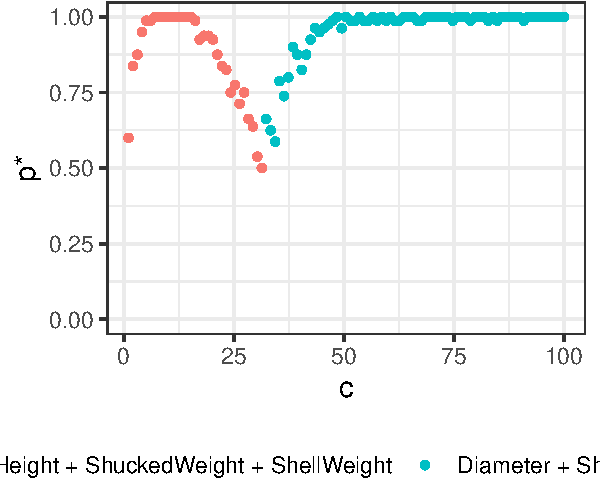
\includegraphics{ReportTemplateBasic1_files/figure-latex/unnamed-chunk-4-1.pdf}

\begin{Shaded}
\begin{Highlighting}[]
\NormalTok{p_select_churchplot=}\KeywordTok{ggplot}\NormalTok{(p_select_church1,}\KeywordTok{aes}\NormalTok{(KoordinaterX,KoordinaterY))}
\NormalTok{p_select_churchplot}\OperatorTok{+}\KeywordTok{geom_point}\NormalTok{(}\KeywordTok{aes}\NormalTok{(}\DataTypeTok{color=}\NormalTok{Stilgruppering))}
\end{Highlighting}
\end{Shaded}

\includegraphics{ReportTemplateBasic1_files/figure-latex/unnamed-chunk-5-1.pdf}

\begin{Shaded}
\begin{Highlighting}[]
\NormalTok{p_select_churchyard=}\StringTok{ }\NormalTok{master_churchyard }\OperatorTok
\KeywordTok{select}\NormalTok{(Plats,KoordinaterX,KoordinaterY,Stilgruppering)}
\NormalTok{p_select_churchyard1=p_select_churchyard }\OperatorTok
\KeywordTok{filter}\NormalTok{(Stilgruppering}\OperatorTok{==}\StringTok{'RAK'} \OperatorTok{|}\StringTok{ }\NormalTok{Stilgruppering}\OperatorTok{==}\StringTok{'Pr2'} \OperatorTok{|}\NormalTok{Stilgruppering}\OperatorTok{==}\StringTok{'Pr3'} \OperatorTok{|}\NormalTok{Stilgruppering}\OperatorTok{==}\StringTok{'Pr4'}\OperatorTok{|}\NormalTok{Stilgruppering}\OperatorTok{==}\StringTok{'Pr5'}\OperatorTok{|}\NormalTok{Stilgruppering}\OperatorTok{==}\StringTok{'FP'}\OperatorTok{|}\NormalTok{Stilgruppering}\OperatorTok{==}\StringTok{'Pr1'}\NormalTok{) }
\NormalTok{count_churchyard=}\KeywordTok{table}\NormalTok{(p_select_churchyard1}\OperatorTok{$}\NormalTok{Stilgruppering)}
\KeywordTok{barplot}\NormalTok{(count_church, }\DataTypeTok{main=}\StringTok{"stone in churchyard"}\NormalTok{,}\DataTypeTok{xlab=}\StringTok{"period"}\NormalTok{)}
\end{Highlighting}
\end{Shaded}

\includegraphics{ReportTemplateBasic1_files/figure-latex/unnamed-chunk-6-1.pdf}

\begin{Shaded}
\begin{Highlighting}[]
\NormalTok{p_select_churchyardplot=}\KeywordTok{ggplot}\NormalTok{(p_select_churchyard1,}\KeywordTok{aes}\NormalTok{(KoordinaterX,KoordinaterY))}
\NormalTok{p_select_churchyardplot}\OperatorTok{+}\KeywordTok{geom_point}\NormalTok{(}\KeywordTok{aes}\NormalTok{(}\DataTypeTok{color=}\NormalTok{Stilgruppering))}
\end{Highlighting}
\end{Shaded}

\includegraphics{ReportTemplateBasic1_files/figure-latex/unnamed-chunk-7-1.pdf}

Summary:

\begin{itemize}
\tightlist
\item
  The data cames from \ldots{}
\item
  The data is/is not valid because \ldots{}
\item
  Possible issues include \ldots{}
\item
  Each row represents \ldots{}
\item
  Each column represents \ldots{}
\end{itemize}

\hypertarget{research-question-1}{%
\subsection{Research Question 1}\label{research-question-1}}

Insert text and analysis.

Summary:

\hypertarget{research-question-2}{%
\subsection{Research Question 2}\label{research-question-2}}

Insert text and analysis.

Summary:

\hypertarget{references-if-needed}{%
\section{References (if needed)}\label{references-if-needed}}

Style: APA


\end{document}
